\begin{enumerate}[label=\thesection.\arabic*.,ref=\thesection.\theenumi]
\numberwithin{equation}{enumi}
\item For a unity feedback system shown in Fig \ref{fig:ee18btech11050_fig1}

\begin{figure}
    \begin{center}
        \tikzstyle{block} = [draw, rectangle, 
        minimum height=3em, minimum width=6em]
        \tikzstyle{sum} = [draw, circle, node distance=1cm]
        \tikzstyle{input} = [coordinate]
        \tikzstyle{output} = [coordinate]
        \tikzstyle{pinstyle} = [pin edge={to-,thin,black}]
        \begin{tikzpicture}[auto, node distance=2cm,>=latex']
            \node [input, name=input] {};
            \node [sum, right of=input] (sum) {X};
            \node [block, right of=sum, %pin={[pinstyle]above:},
                    ] (system) {$G(s)$};
            \node [output, right of=system] (output) {};
            \node [output,below of=system] (measurements) {};

            \draw [draw,->] (input) -- node {$R(s)$} (sum);
            \draw [->] (sum) -- node[anchor=north] {$-$} (system);
            \draw [->] (system) -- node [name=y] {$Y(s)$}(output);
            \draw [-] (y) |- (measurements);
            \draw [->] (measurements) -| node[pos=0.99] {$+$} 
                node [near end] {} (sum);
        \end{tikzpicture}

    \end{center}
    \caption{}
    \label{fig:ee18btech11050_fig1}
\end{figure}

having transfer function
\begin{align}
    G(s) = \frac{K}{(s+3)(s+9)(s+15)}
    \label{eq:ee18btech11050_1}
\end{align}
design the value of gain(K), for a gain margin of 50 dB.

\item \solution

Gain Margin:
\begin{align}
    GM = -20\log{|G(j\omega_{pc})|}
    \label{eq:ee18btech11050_2}
\end{align}
where, $\omega_{pc}$ is the phase cross-over frequency, at which
\begin{align}
    \angle {G(j \omega_{pc})} = -180 \degree
    \label{eq:ee18btech11050_3}
\end{align}
First substitute, 
\begin{align}
    s = j\omega
\end{align}
\begin{align}
    \implies G(j\omega) = \frac{K}{(-27\omega^2+405)+j(-\omega^3+207\omega)}
    \label{eq:ee18btech11050_4}
\end{align}
Now the phase will be
\begin{align}
    \angle{G(j\omega)} = -\tan^{-1}(\frac{-\omega^3+207\omega}{-27\omega^2+405})
    \label{eq:ee18btech11050_5}
\end{align}
Solving for $\angle{G(j\omega)}=-180\degree$ gives
\begin{align}
  \omega_{pc} = 14.3875
\end{align}
Magnitude :
\begin{align}
    |G(j\omega)| = \frac{K}{\sqrt{(\omega^2+9)}\sqrt{(\omega^2+81)}\sqrt{(\omega^2+225)}}
    \label{eq:ee18btech11050_6}
\end{align}
Substituting value of $\omega_{pc}$ in \eqref{eq:ee18btech11050_2} gives
\begin{align}
    K = 16.406
\end{align}
This can be verified from fig \ref{fig:ee18btech11050_fig2}
\begin{figure}[!ht]
\centering
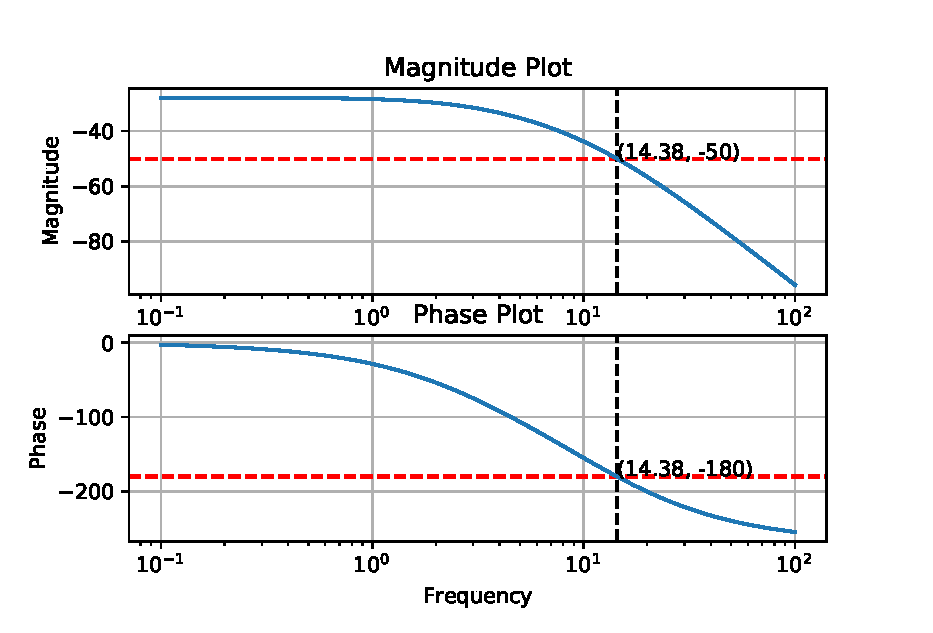
\includegraphics[width=\columnwidth]{./figs/ee18btech11050_1.eps}
\caption{}
\label{fig:ee18btech11050_fig2}
\end{figure}
The following code generates Fig. \ref{fig:ee18btech11050_fig2}
\begin{lstlisting}
codes/ee18btech11050_1.py
\end{lstlisting}
\item Design the value gain (K) for a phase margin of 40\degree.
\item \solution

Phase Margin:
\begin{align}
    PM = 180\degree + \phi_{gc}
    \label{eq:ee18btech11050_7}
\end{align}
where $\phi_{gc}$ is the phase angle at the gain cross over frequency $\omega_{gc}$.
At gain cross over frequency,
\begin{align}
    |G(j\omega_{gc})| = 1
    %\label{eq:ee18btech11050_22}
\end{align}
\begin{align}
    \implies -20\log{|G(j\omega_{gc})|} = 0
    \label{eq:ee18btech11050_111}
\end{align}

Given,
\begin{align}
    PM = 40\degree = 180\degree + \phi_{gc}
    \label{eq:ee18btech11050_8}
\end{align}
\begin{align}
    \implies \phi_{gc} = -140\degree = \angle{G(j\omega_{gc})}
\end{align}
From \eqref{eq:ee18btech11050_5} 
\begin{align}
    \angle{G(j\omega_{gc})} = -\tan^{-1}(\frac{-\omega_{gc}^3+207\omega_{gc}}{-27\omega_{gc}^2+405})
    \label{eq:ee18btech11050_9}
\end{align}
\begin{align}
    \implies \omega_{gc} = 8.09623
    \label{eq:ee18btech11050_10}
\end{align}

Substituting this value in \eqref{eq:ee18btech11050_111}, we get
\begin{align}
    20\log{K} = 65.016
\end{align}
\begin{align}
    \implies K = 1781.56
    \label{eq:ee18btech11050_12}
\end{align}

This again can be verified from fig \ref{fig:ee18btech11050_fig3}.
The following code generates Fig. \ref{fig:ee18btech11050_fig3}
\begin{lstlisting}
codes/ee18btech11050_2.py
\end{lstlisting}
\begin{figure}[!ht]
\centering
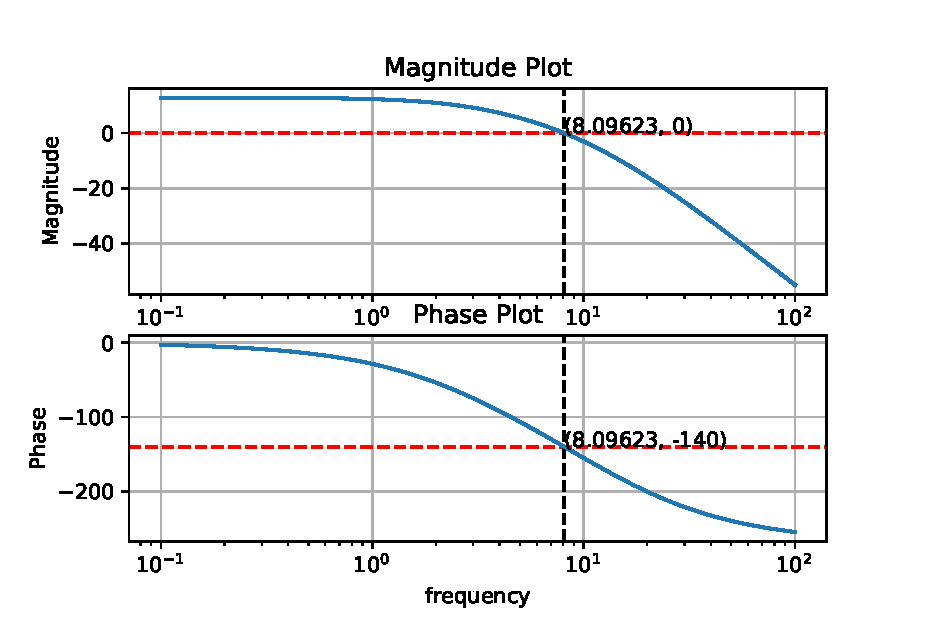
\includegraphics[width=\columnwidth]{./figs/ee18btech11050_2.eps}
\caption{}
\label{fig:ee18btech11050_fig3}
\end{figure}

\item Design the value of gain (K) to yield maximum peak overshoot of 20\% for a step input.

\item \solution
Closed loop transfer function:
\begin{align}
    T(s) = \frac{G(s)}{1+G(s)H(s)}
\end{align}
where H(s) = 1
\begin{align}
    \implies T(s) = \frac{K}{(s+3)(s+6)(s+15)+K}
    \label{eq:ee18btech11050_13}
\end{align}
Output will be:
\begin{align}
    \implies Y(s) = \frac{1}{s}\frac{K}{(s+3)(s+6)(s+15)+K}
    \label{eq:ee18btech11050_14}
\end{align}

Maximum peak overshoot :
\begin{align}
    M_p = \frac{y(t_p) - y(\infty)}{y(\infty)}
    \label{eq:ee18btech11050_15}
\end{align}
which is given as 20\%.
Here, $t_p$ is the peak time. Solving this, we get
\begin{align}
    \implies \frac{y(t_p)}{y(\infty)} = 1.2
    \label{eq:ee18btech11050_18}
\end{align}
Plotting y(t) for different values of K, we choose the value of K, which gives the above ratio, which is verfied from fig \ref{fig:ee18btech11050_fig4}.
Thus, we get 
\begin{align}
    t_p = 0.505
    \label{eq:ee18btech11050_16}
\end{align}
\begin{align}
    \implies K = 928.035
    \label{eq:ee18btech11050_17}
\end{align}



\begin{figure}[!ht]
\centering
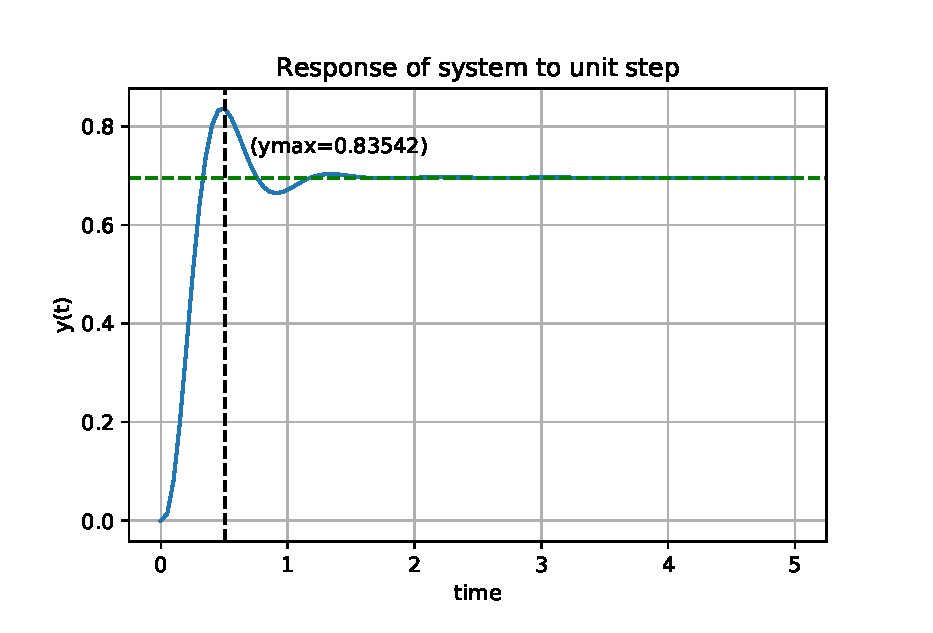
\includegraphics[width=\columnwidth]{./figs/ee18btech11050_3.eps}
\caption{}
\label{fig:ee18btech11050_fig4}
\end{figure}

The following code generates fig \ref{fig:ee18btech11050_fig4}
\begin{lstlisting}
codes/ee18btech11050_3.py
\end{lstlisting}

\end{enumerate}
